% ==================== 3 计算晶体消光系数 ====================
\section{计算晶体消光系数}

\subsection{两部分工作的区分}

电子衍射模拟实际上包含两个相对独立的部分：第一部分计算晶面的结构因子，也就是本文所说的“消光系数”，用来判断哪些晶面允许衍射、哪些晶面消光；第二部分建立二维倒易点阵，计算衍射点的坐标并绘制电子衍射图。两部分使用的 Origin 表格并不相同：消光系数表的表头是 $f,x,y,z,h,k,l,\text{phase},\cos,\sin,I$，而衍射图表表头是 $r_1,r_2,\theta,m,n,x,y,I,h,k,l$。如果把两张表混在一起，就会出现“用衍射图的列去算结构因子”或“用原子坐标列去画斑点”的错误。

本章完成第一部分：先从 Si.cif 提取 8 个原子的分数坐标，再在 Origin 中按 $f=14$ 计算每个晶面的相位、实部、虚部和 $|F|^2$，最后用 110 反射验证金刚石结构的消光规律。第 4 章再完成第二部分，建立二维倒易点阵并绘制五个带轴的衍射图。

表 \ref{tab:two-tables} 对比了两张表的用途和列名，可作为插图时区分图片的依据：图 \ref{fig:structure-factor}(b)(c)(d) 的表格属于消光系数表，第 4 章的衍射图表格属于另一张表。

\begin{table}[H]
  \centering
  \caption{消光系数计算表与衍射图绘制表的区别}
  \label{tab:two-tables}
  \small
  \setlength{\tabcolsep}{4pt}
  \renewcommand{\arraystretch}{1.08}
  \begin{tabular}{p{0.16\linewidth}p{0.44\linewidth}p{0.28\linewidth}}
    \toprule
    用途 & 典型列名 & 输出 \\
    \midrule
    消光系数计算 & $f,x,y,z,h,k,l,\text{phase},\cos,\sin,I$ & 每个晶面的 $|F|^2$，判断是否消光 \\
    衍射图绘制 & $r_1,r_2,\theta,m,n,x,y,I,h,k,l$ & 每个斑点的坐标 $(x,y)$ 与点阵图 \\
    \bottomrule
  \end{tabular}
\end{table}

\subsection{从 CIF 到原子坐标}

计算结构因子需要晶胞内全部原子的分数坐标。图 \ref{fig:cif-export} 给出了从 CIF 文件提取坐标的过程。首先把 Si.cif 拖入 VESTA，软件会显示金刚石型的球棍模型，如图 \ref{fig:cif-export}(a) 所示。然后在 \texttt{Options} 中把原子坐标的写出方式设为 Fractional coordinates（分数坐标），如图 \ref{fig:cif-export}(b) 所示；接着选择 \texttt{File $\rightarrow$ Export Data}，把结构导出为 P1 对称性的 \texttt{.p1} 文件，如图 \ref{fig:cif-export}(c)(d) 所示。P1 文件把所有对称操作展开，直接列出晶胞内全部原子的坐标，便于复制到 Origin。

用记事本打开导出的 \texttt{Si.p1} 文件，可以看到晶胞参数和 \texttt{Direct} 坐标块，如图 \ref{fig:cif-export}(e) 所示。文件中的 $a=5.4306$~\AA，与题目给定的 5.43~\AA 只差 $6\times10^{-4}$~\AA，属于 CIF 数据的有效数字差异；本文统一按 5.43~\AA 计算。坐标块列出 8 个 Si 原子，其分数坐标与表 \ref{tab:si-atoms} 完全一致，可直接作为结构因子计算的输入。

\begin{figure}[H]
  \centering
  \begin{subfigure}[t]{0.60\linewidth}
    \centering
    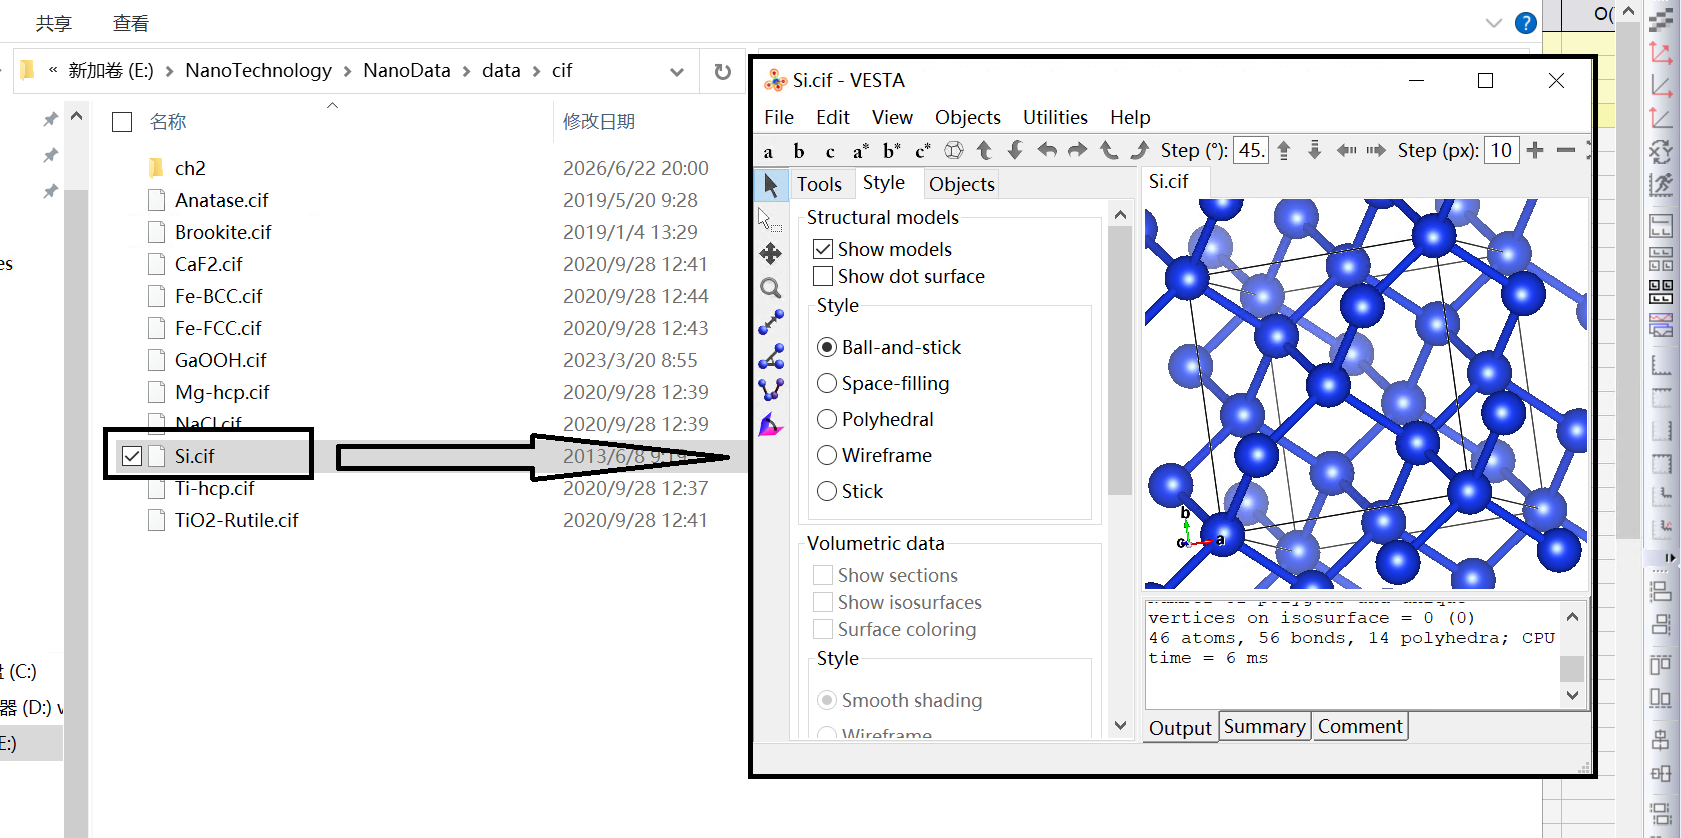
\includegraphics[width=\linewidth]{proc/p01.png}
    \caption{把 Si.cif 拖入 VESTA}
    \label{fig:cif-export-a}
  \end{subfigure}\hfill
  \begin{subfigure}[t]{0.34\linewidth}
    \centering
    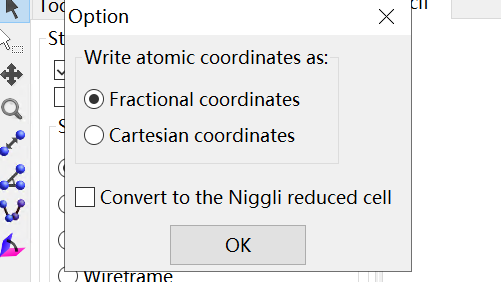
\includegraphics[width=\linewidth]{proc/p02.png}
    \caption{选择分数坐标}
    \label{fig:cif-export-b}
  \end{subfigure}

  \vspace{0.3em}
  \begin{subfigure}[t]{0.26\linewidth}
    \centering
    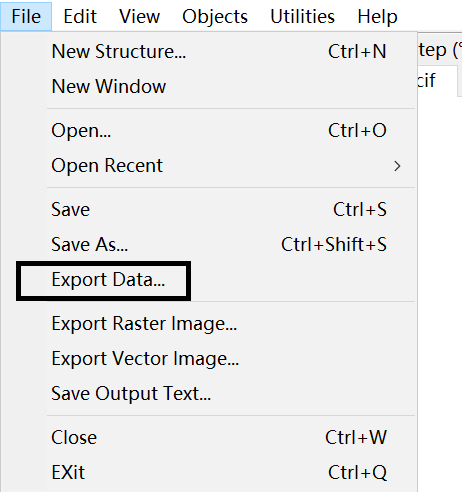
\includegraphics[width=\linewidth]{proc/p03.png}
    \caption{File $\rightarrow$ Export Data}
    \label{fig:cif-export-c}
  \end{subfigure}\hfill
  \begin{subfigure}[t]{0.38\linewidth}
    \centering
    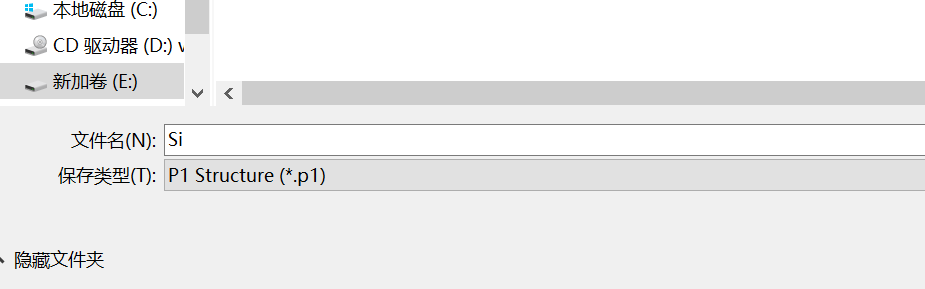
\includegraphics[width=\linewidth]{proc/p04.png}
    \caption{导出为 P1 结构}
    \label{fig:cif-export-d}
  \end{subfigure}

  \vspace{0.3em}
  \begin{subfigure}[t]{0.86\linewidth}
    \centering
    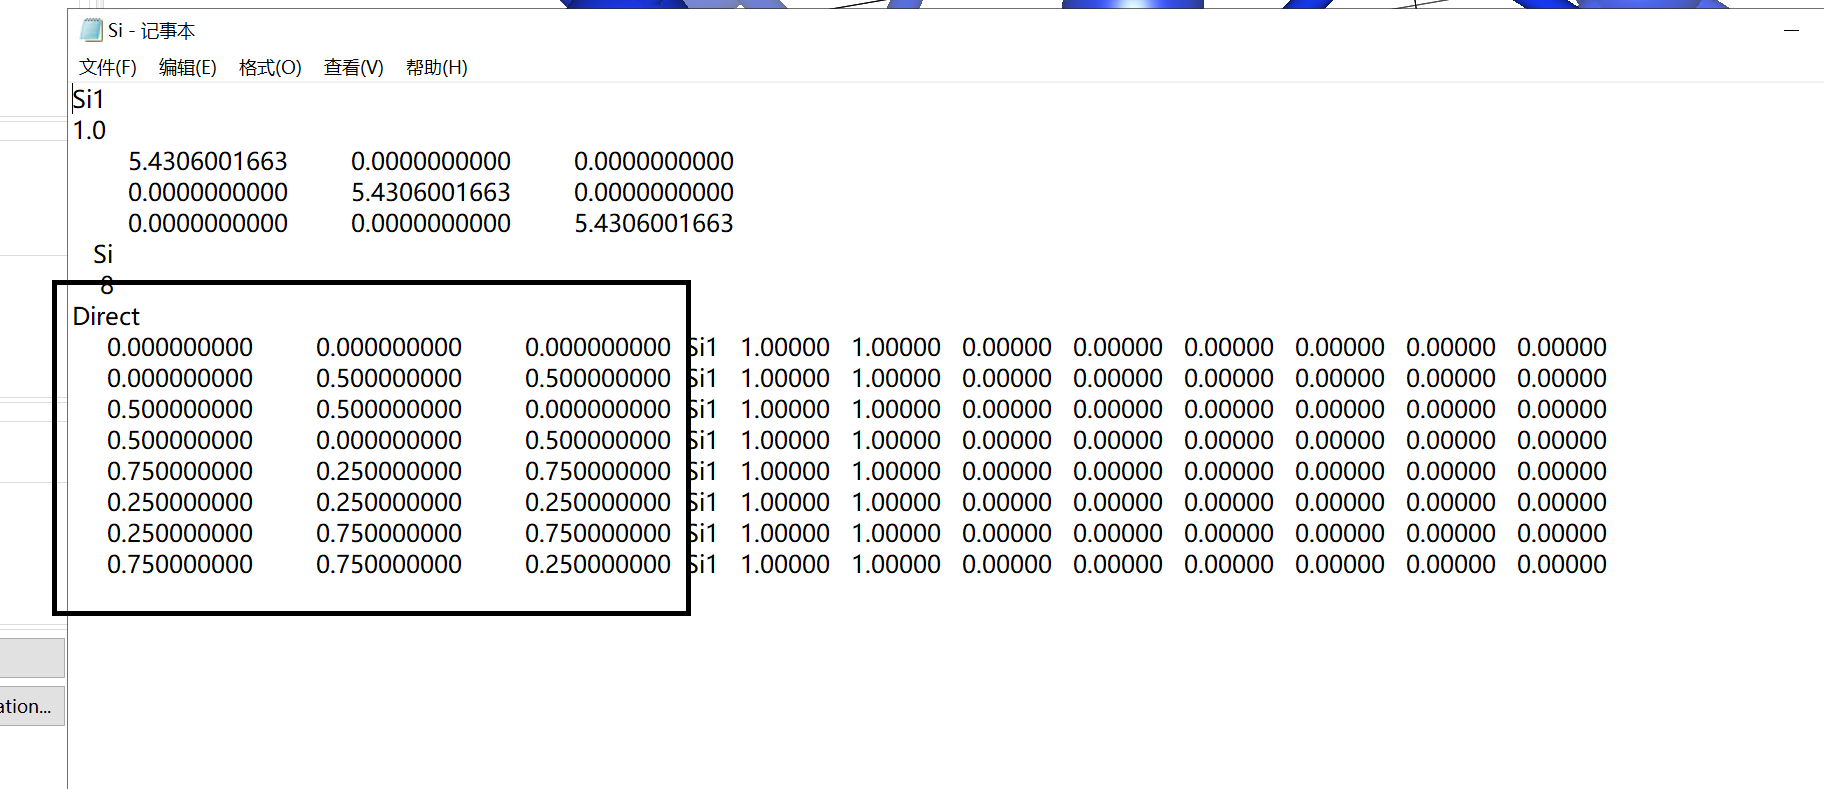
\includegraphics[width=\linewidth]{proc/p05.png}
    \caption{用记事本读取 \texttt{Direct} 坐标块}
    \label{fig:cif-export-e}
  \end{subfigure}
  \caption{从 Si.cif 提取 8 个原子分数坐标：(a) VESTA 显示金刚石结构；(b) 设置为分数坐标；(c)(d) 导出 P1 文件；(e) 记事本中的晶胞参数与 \texttt{Direct} 坐标块。}
  \label{fig:cif-export}
\end{figure}

\subsection{结构因子与消光系数}
\label{sec:f14}

运动学近似下，晶面 $(hkl)$ 的衍射强度正比于结构因子模的平方：
\begin{equation}
I(hkl)\propto|F(hkl)|^2,\qquad
F(hkl)=\sum_{j=1}^{N}g_jt_j(s)f_j(s)\exp\left[2\pi i(hx_j+ky_j+lz_j)\right].
\label{eq:extinction-F}
\end{equation}
当 $|F(hkl)|^2=0$ 时，该晶面不产生衍射，称为消光。本文按课程习惯，把由结构因子得到的相对强度因子 $|F(hkl)|^2$ 称为该晶面的“消光系数”；严格地说，它是运动学近似下的结构因子平方，而不是动力学理论中的消光系数。

图 \ref{fig:structure-factor}(a) 给出了结构因子公式，图 \ref{fig:structure-factor}(b) 给出了 $f=14$ 和 8 个原子的分数坐标，图 \ref{fig:structure-factor}(c)(d) 给出了相位差、实部、虚部和强度的计算。图 \ref{fig:structure-factor}(b)(c)(d) 的表格表头为 $f,x,y,z,h,k,l,\text{phase},\cos,\sin,I$，对应 A--K 列；它只用于消光系数计算，不用于画衍射图。

把表 \ref{tab:si-atoms} 的 8 行坐标放在一起，令
\begin{lstlisting}
phase = 360*(E*B + F*C + G*D)
real  = A*COS(H)
imag  = A*SIN(H)
I     = (TOTAL(I))^2 + (TOTAL(J))^2
\end{lstlisting}
其中 A 为 $f=14$，B、C、D 为原子的 $x,y,z$，E、F、G 为 $h,k,l$，H 为相位。每个衍射点需要 8 行原子坐标；\texttt{TOTAL} 对这 8 行求和，得到 $\sum f\cos\phi$ 和 $\sum f\sin\phi$，再平方相加即得 $|F|^2$。若一次计算多个衍射点，应把每个点的 8 行作为一个块，用 \texttt{SUM} 指定块范围，或增加“斑点编号”列后用 \texttt{TOTALIF} 按编号分组，避免把不同斑点的原子混在一起。

\begin{figure}[H]
  \centering
  \begin{subfigure}[t]{0.96\linewidth}
    \centering
    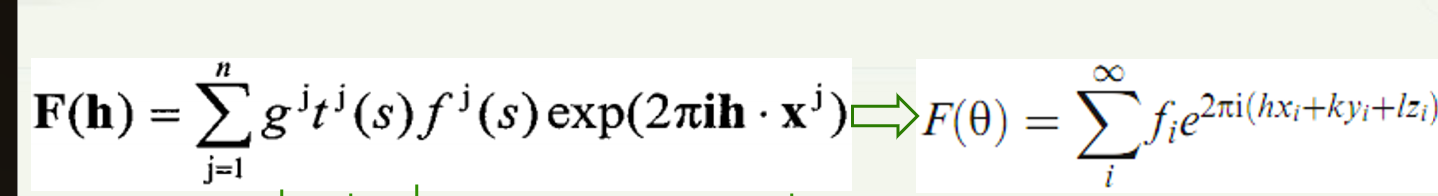
\includegraphics[width=\linewidth]{proc/p16.png}
    \caption{结构因子公式}
    \label{fig:structure-factor-a}
  \end{subfigure}

  \vspace{0.25em}
  \begin{subfigure}[t]{0.62\linewidth}
    \centering
    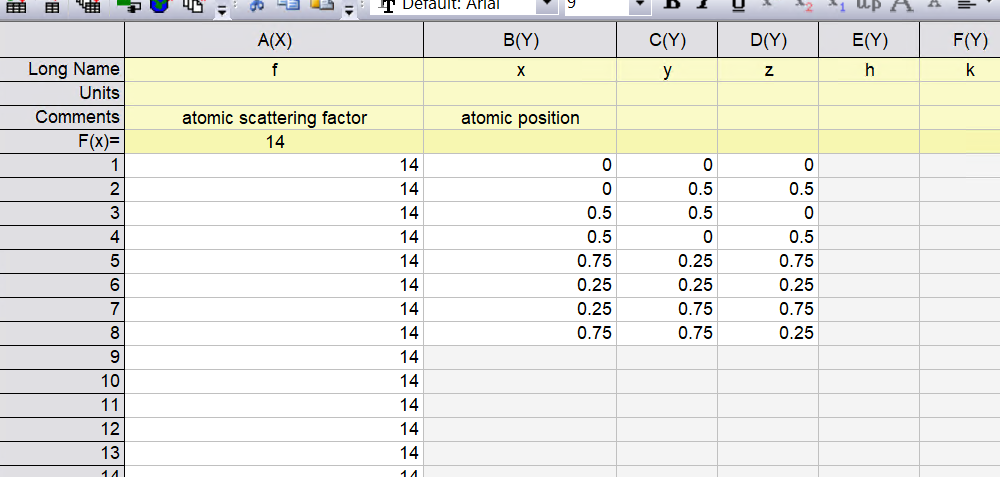
\includegraphics[width=\linewidth]{proc/p17.png}
    \caption{$f=14$（Si 的原子序数）与 8 个原子坐标}
    \label{fig:structure-factor-b}
  \end{subfigure}\hfill
  \begin{subfigure}[t]{0.32\linewidth}
    \centering
    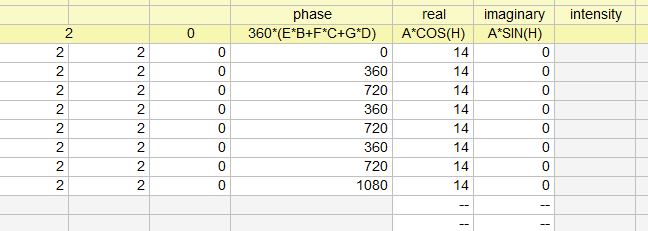
\includegraphics[width=\linewidth]{proc/p18.png}
    \caption{相位差公式}
    \label{fig:structure-factor-c}
  \end{subfigure}

  \vspace{0.25em}
  \begin{subfigure}[t]{0.36\linewidth}
    \centering
    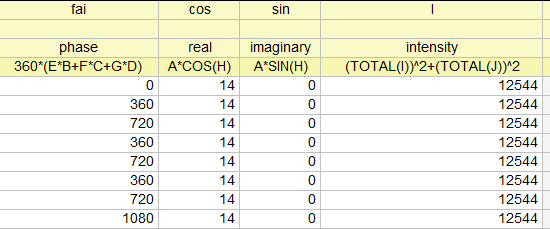
\includegraphics[width=\linewidth]{proc/p19.png}
    \caption{强度公式与结果}
    \label{fig:structure-factor-d}
  \end{subfigure}
  \caption{消光系数（结构因子）的计算：(a) $F(h)=\sum g^jt^j(s)f^j(s)\exp(2\pi i\bm{h}\cdot\bm{x}^j)$；(b) $f=14$ 和 8 个原子的分数坐标，表头为 $f,x,y,z,h,k,l,\text{phase},\cos,\sin,I$；(c) 相位差 $360^\circ(hx+ky+lz)$ 及实部、虚部；(d) 强度 $(\sum\mathrm{real})^2+(\sum\mathrm{imag})^2$。}
  \label{fig:structure-factor}
\end{figure}

图 \ref{fig:structure-factor}(b) 中的 $f=14$ 不是一个随意设定的常数，而是 Si 原子散射因子的前向散射值。原子散射因子 $f$（严格写作 $f(s)$，$s=\sin\theta/\lambda$）表示一个原子在给定方向上的散射振幅与一个自由电子散射振幅之比，量纲为 1；当散射角趋于零时，各电子的散射波完全同相叠加，$f(0)$ 近似等于原子的核外电子数，即原子序数 $Z$。Si 的 $Z=14$，所以模板取 $f=14$，相当于采用 $f(0)$ 这一上限值。真实晶体的 $f(s)$ 随 $\sin\theta/\lambda$ 增大而单调下降，还要乘上温度因子 $t(s)=\exp(-Bs^2)$（第 \ref{sec:cromer-mann} 节 PDF 卡片用的 Cromer--Mann $f(s)$ 就是这种角度依赖的定量表述），因此固定 $f=14$ 属于运动学近似下的最简处理。

这一简化对“是否消光”的判断是充分的：$F(hkl)=0$ 来自晶胞内各原子相位项的完全抵消，与 $f$ 取何值无关，所以用 $f=14$ 算出的零强度点，在真实晶体中同样消光。但它对未消光反射的相对强度只是近似：高角反射的真实 $f(s)$ 已明显小于 14，其强度会被本模板高估，这与表 \ref{tab:pdf-card} 中 $f=14$ 与 $f(s)$ 两列强度的差异是同一原因。

\subsection{110 反射的消光验证}

图 \ref{fig:extinction} 以 110 反射为例验证消光。110 的 $h,k,l$ 为奇偶混合，按第 1 章的规则应有 $F=0$。在表格中输入 $h=k=1$、$l=0$ 后，相位依次为 $0^\circ,180^\circ,360^\circ,\ldots$，8 个原子的实部两两抵消，最终强度约为 $4.7\times10^{-29}$，在数值上就是零。这个结果说明：几何点阵中虽然会出现 110 的位置，但结构因子会使该点消光；实际电子衍射花样中不会看到这个斑点。第 4 章绘制衍射图时，应把这类消光点删除或置零，不能把它们当作真实斑点。

\begin{figure}[H]
  \centering
  \begin{subfigure}[t]{0.20\linewidth}
    \centering
    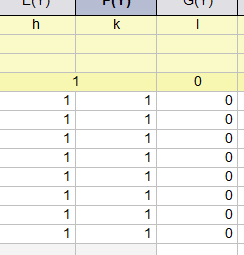
\includegraphics[width=\linewidth]{proc/p20.png}
    \caption{输入 $hkl=110$}
    \label{fig:extinction-a}
  \end{subfigure}\hfill
  \begin{subfigure}[t]{0.46\linewidth}
    \centering
    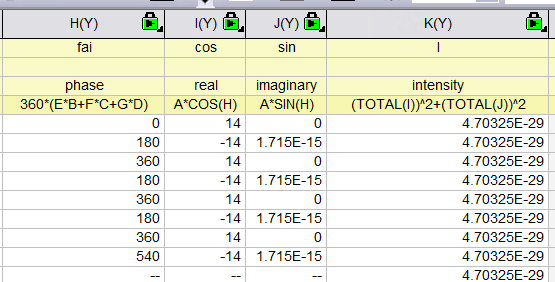
\includegraphics[width=\linewidth]{proc/p21.png}
    \caption{强度全部消光}
    \label{fig:extinction-b}
  \end{subfigure}
  \caption{110 反射的消光验证：(a) 输入 $h=k=1,l=0$；(b) 实部正负抵消，强度约 $4.7\times10^{-29}$。}
  \label{fig:extinction}
\end{figure}

\subsection{单晶硅的消光规律}

把上述计算用于一组典型晶面，可得到表 \ref{tab:extinction-examples}。金刚石结构的消光规律可以归纳为：
\begin{itemize}[leftmargin=2em,itemsep=1pt]
  \item $h,k,l$ 奇偶混合：$|F|^2=0$，消光；
  \item $h,k,l$ 全为偶数且 $h+k+l=4n+2$：$|F|^2=0$，消光；
  \item $h,k,l$ 全为奇数：$|F|^2=32f^2=6272$（$f=14$），允许；
  \item $h,k,l$ 全为偶数且 $h+k+l=4n$：$|F|^2=64f^2=12544$（$f=14$），允许且较强。
\end{itemize}
因此，Si 的允许反射为 111、220、311、400、331、422、511/333、440、531、620 等，而 100、110、200、222、420、600 等消光。第 4 章在每个带轴的几何点阵中会保留所有 $m,n$ 格点，但只有表 \ref{tab:extinction-examples} 中“允许”的格点才是真实衍射斑；实际绘图时应按消光系数表把这些点筛选出来。

\begin{table}[H]
  \centering
  \caption{单晶硅典型晶面的结构因子与消光判断（$f=14$）}
  \label{tab:extinction-examples}
  \small
  \setlength{\tabcolsep}{5pt}
  \renewcommand{\arraystretch}{1.03}
  \begin{tabular}{cccccl}
    \toprule
    $hkl$ & $h+k+l$ & 奇偶性 & $|F|^2$ & 判断 & 说明 \\
    \midrule
    111 & 3 & 全奇 & 6272  & 允许 & $32f^2$ \\
    200 & 2 & 全偶，$4n+2$ & 0 & 消光 & $h+k+l=2$ \\
    220 & 4 & 全偶，$4n$ & 12544 & 允许 & $64f^2$ \\
    222 & 6 & 全偶，$4n+2$ & 0 & 消光 & $h+k+l=6$ \\
    311 & 5 & 全奇 & 6272  & 允许 & $32f^2$ \\
    400 & 4 & 全偶，$4n$ & 12544 & 允许 & $64f^2$ \\
    331 & 7 & 全奇 & 6272  & 允许 & $32f^2$ \\
    420 & 6 & 全偶，$4n+2$ & 0 & 消光 & $h+k+l=6$ \\
    422 & 8 & 全偶，$4n$ & 12544 & 允许 & $64f^2$ \\
    511/333 & 7/9 & 全奇 & 6272 & 允许 & $32f^2$ \\
    440 & 8 & 全偶，$4n$ & 12544 & 允许 & $64f^2$ \\
    531 & 9 & 全奇 & 6272 & 允许 & $32f^2$ \\
    600 & 6 & 全偶，$4n+2$ & 0 & 消光 & $h+k+l=6$ \\
    620 & 8 & 全偶，$4n$ & 12544 & 允许 & $64f^2$ \\
    \bottomrule
  \end{tabular}
\end{table}
